\documentclass{CE295_HW_template}

\newcommand{\hmwkNum}{3}
\newcommand{\hmwkTitle}{HW \hmwkNum: Optimal Economic Dispatch in Distribution Feeders with Renewables}
\newcommand{\hmwkAuthorName}{Carlin Liao}
\newcommand{\SID}{24358933}

\title{
\vspace{-0.5cm}
\textbf{\hmwkTitle}
\author{} % Leave this blank
\date{} % Leave this blank
\vspace{-1cm}
}

%% Do not edit unless you really know what you are doing.
\documentclass[english]{article}
\usepackage[T1]{fontenc}
\usepackage[latin9]{inputenc}
\usepackage{textcomp}
\usepackage{relsize}

\makeatletter

%%%%%%%%%%%%%%%%%%%%%%%%%%%%%% User specified LaTeX commands.
\def\labnb{0}
\usepackage{hyperref} 
\usepackage{ulem}
\usepackage{latexsym}
\usepackage{amssymb}
\usepackage{amsmath}
\usepackage{amsfonts}
\usepackage{color, colortbl}
\usepackage{graphicx}
\usepackage{lastpage}
\usepackage[framed,numbered,autolinebreaks,useliterate]{mcode}

\newcommand{\red}[1]{{\color{red}#1}}
\newcommand{\blue}[1]{{\color{blue}#1}}
\newcommand{\green}[1]{{\color{green}#1}}

%%%%%%%%%%%%%%%%%%%%%%%%%%%%%%%%%%%%%%%%%%%%%%
\begin{document}
\maketitle
\thispagestyle{fancy}

%---------------
% PROBLEM 1
%---------------

\begin{Problem}[Network Parameters]

\begin{enumerate}
\renewcommand{\theenumi}{(\alph{enumi})}
    \item As follows:
        \begin{figure}[!htbp]
            \centering
            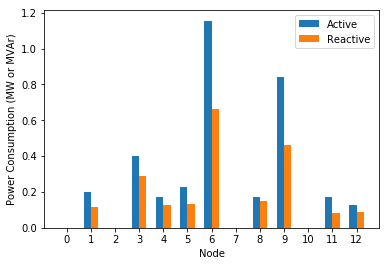
\includegraphics[width=30em]{"imgs/[3] HW3"/1a.png}
            \caption{Active and reactive power consumption}
            \label{fig:1a}
        \end{figure} 
    \item Adjacency matrix $A$ is as follows: \begin{verbatim}
1  1  0  0  0  0  0  0  0  0  0  0  0 
0  0  1  0  1  0  1  0  0  0  0  0  0 
0  0  0  1  0  0  0  0  0  0  0  0  0 
0  0  0  0  0  0  0  0  0  0  0  0  0 
0  0  0  0  0  1  0  0  0  0  0  0  0 
0  0  0  0  0  0  0  0  0  0  0  0  0 
0  0  0  0  0  0  0  1  1  0  1  0  0 
0  0  0  0  0  0  0  0  0  0  0  0  0 
0  0  0  0  0  0  0  0  0  1  0  0  0 
0  0  0  0  0  0  0  0  0  0  0  0  0 
0  0  0  0  0  0  0  0  0  0  0  1  1 
0  0  0  0  0  0  0  0  0  0  0  0  0 
0  0  0  0  0  0  0  0  0  0  0  0  0
    \end{verbatim}
\end{enumerate}


\end{Problem}

%---------------
% PROBLEM 2
%---------------

\begin{Problem}[Balancing Supply \& Demand without a Network]

\begin{enumerate}
\renewcommand{\theenumi}{(\alph{enumi})}
    \item The optimization variables are $p_j$, $q_j$, $s_j$ for all $j$ in $\mathcal{N}$.
    
    \item $$\min_{p_j, q_j, s_j \forall j \in \matcal{N}} c^T s$$
    
    \item
    \begin{align*}
        s_j &\leq s_{j,\max} & \forall j \in \matcal{N} \qquad& \text{Apparent power limits} \\
        \sum_{j \in \mathcal{N}} q_j &= \sum_{j \in \mathcal{N}} l_j^Q && \text{Balance generation with consumption} \\
        \sum_{j \in \mathcal{N}} p_j &= \sum_{j \in \mathcal{N}} l_j^P && \text{Balance generation with consumption} \\
        p_j &\geq 0 & \forall j \in \matcal{N} \qquad & \text{Non-negative power generation} \\
        q_j &\geq 0 & \forall j \in \matcal{N} \qquad& \text{Non-negative power generation} \\
        s_j &= \|[p_j, q_j]\|_2 & \forall j \in \matcal{N}  \qquad& \text{Apparent power} 
    \end{align*}
    \item The norm term makes this program quadratic, with the equality constraint on the norm disqualifying it from being convex because although it's convex it's not an affine expression. When we relax that to an inequality, all of our equality constraints are now affine and our inequality constraints convex functions, so we now have a convex program.
    \item \begin{verbatim}
Minimum Generating Cost : 255.36 USD
 
Node 0 [Grid]  Gen Power : p_0 = 0.901 MW | q_0 = 0.546 MW | s_0 = 1.054 MW
Node 3 [Gas]   Gen Power : p_3 = 0.000 MW | q_3 = 0.000 MW | s_3 = 0.000 MW
Node 9 [Solar] Gen Power : p_9 = 2.565 MW | q_9 = 1.556 MW | s_9 = 3.000 MW
 
Total active power   : 3.466 MW   consumed | 3.466 MW   generated
Total reactive power : 2.102 MVAr consumed | 2.102 MVAr generated
Total apparent power : 4.063 MVA  consumed | 4.054 MVA  generated
    \end{verbatim}
\end{enumerate}

\end{Problem}

%---------------
% PROBLEM 3
%---------------

\begin{Problem}[Add Line Power Flows]

\begin{enumerate}
\renewcommand{\theenumi}{(\alph{enumi})}
    \item Again, the optimization variables are $p_j$, $q_j$, $s_j$, with the new variables $P_{ij}$, $Q_{ij}$ for all $i$ in $\rho(j)$ and $j$ in $\mathcal{N}$.
    
    \item
    \begin{align*}
        P_{0,0} &= 0 && \text{Boundary condition} \\
        Q_{0,0} &= 0 && \text{Boundary condition} \\
        s_j &\leq s_{j,\max} & \forall j \in \matcal{N} \qquad& \text{Apparent power limits} \\
        p_j &\geq 0 & \forall j \in \matcal{N} \qquad & \text{Non-negative power generation} \\
        q_j &\geq 0 & \forall j \in \matcal{N} \qquad& \text{Non-negative power generation} \\
        s_j &= \|[p_j, q_j]\|_2 & \forall j \in \matcal{N}  \qquad& \text{Apparent power} \\
        P_{ij} &= (l_j^P-p_j) + \sum_{k\in \mathcal{N}} A_{jk} P_{jk} & \forall j \in \matcal{N},\ i = \rho(j)  \qquad& \text{Line active power balance} \\
        Q_{ij} &= (l_j^Q-q_j) + \sum_{k\in \mathcal{N}} A_{jk} Q_{jk} & \forall j \in \matcal{N},\ i = \rho(j)  \qquad& \text{Line reactive power balance}
    \end{align*}
    \item (For full output, see section after the next list item). The minimum and minimizers should be the same because we aren't adding any additional hard constraints to the power generation. Instead, we're merely moving to track and solve for the flow of power throughout the network using the new variables of $P$ and $Q$, but neither are present in the objective function and are merely generated as functions of the original optimization variables $p_j$, $q_j$, and $s_j$. 
    \item The values of the dual variable vector on the constraint $s_j \leq s_{j,\max} \forall j \in \matcal{N}$ are as follows: \begin{verbatim}
[[2.71965205e-09]
 [3.05397381e+02]
 [3.05397381e+02]
 [2.70575918e-09]
 [3.05397381e+02]
 [3.05397381e+02]
 [3.05397381e+02]
 [3.05397381e+02]
 [3.05397381e+02]
 [5.00000000e+01]
 [3.05397381e+02]
 [3.05397381e+02]
 [3.05397381e+02]]\end{verbatim} We note that the dual variable for node 9, the solar capacity, is \$50/MW, so we conclude that increasing the solar capacity by 1 MW decreases total cost by exactly \$50.
\end{enumerate}

\begin{verbatim}
------------------- PROBLEM 3 --------------------
--------------------------------------------------
optimal
Minimum Generating Cost : 255.36 USD
 
Node 0 [Grid]  Gen Power : p_0 = 0.901 MW | q_0 = 0.546 MW | s_0 = 1.054 MW || mu_s0 =   0 USD/MW
Node 3 [Gas]   Gen Power : p_3 = 0.000 MW | q_3 = 0.000 MW | s_3 = 0.000 MW || mu_s4 =   0 USD/MW
Node 9 [Solar] Gen Power : p_9 = 2.565 MW | q_9 = 1.556 MW | s_9 = 3.000 MW || mu_s9 =  50 USD/MW
 
Total active power   : 3.466 MW   consumed | 3.466 MW   generated
Total reactive power : 2.102 MVAr consumed | 2.102 MVAr generated
Total apparent power : 4.063 MVA  consumed | 4.054 MVA  generated
    \end{verbatim}

\end{Problem}

%---------------
% PROBLEM 4
%---------------

\begin{Problem}[The Complete Optimal Economic Dispatch with DistFlow Equation]

\begin{enumerate}
\renewcommand{\theenumi}{(\alph{enumi})}
    \item Now in addition to the variables from Problems 2 and 3, $p_j$, $q_j$, $s_j$, $P_{ij}$, $Q_{ij}$, we also have $V_j$ and $L_{ij}$ for all $i$ in $\rho(j)$ and $j$ in $\mathcal{N}$. 
    \item 
    \begin{align*}
        P_{0,0} &= 0 && \text{Boundary condition} \\
        Q_{0,0} &= 0 && \text{Boundary condition} \\
        V_0 &= 1 && \text{Fix node 0 voltage to be 1 per unit} \\
        L_{0,0} &= 0 && \text{Boundary condition} \\
        s_j &\leq s_{j,\max} & \forall j \in \matcal{N} \qquad& \text{Apparent power limits} \\
        p_j &\geq 0 & \forall j \in \matcal{N} \qquad & \text{Non-negative power generation} \\
        q_j &\geq 0 & \forall j \in \matcal{N} \qquad& \text{Non-negative power generation} \\
        s_j &= \|[p_j, q_j]\| & \forall j \in \matcal{N}  \qquad& \text{Apparent power} \\
        P_{ij} &= (l_j^P-p_j) + r_{ij}L_{ij} + \sum_{k\in \mathcal{N}} A_{jk} P_{jk} & \forall j \in \matcal{N},\ i = \rho(j)  \qquad& \text{Line active power balance} \\
        Q_{ij} &= (l_j^Q-q_j) + x_{ij}L_{ij} + \sum_{k\in \mathcal{N}} A_{jk} Q_{jk} & \forall j \in \matcal{N},\ i = \rho(j)  \qquad& \text{Line reactive power balance} \\
        V_j &= V_i + (r_{ij}^2 + x_{ij}^2)L_{ij} - 2(r_{ij}P_{ij} + x_{ij}Q_{ij}) & \forall j \in \matcal{N},\ i = \rho(j)  \qquad& \text{Voltage balance} \\
        L_{ij} &= \frac{P_{ij}^2 + Q_{ij}^2}{V_j} & \forall j \in \matcal{N},\ i = \rho(j)  \qquad& \text{Line current} \\
        v_\min^2 &\leq V_j & \forall j \in \mathcal{N} \qquad& \text{Voltage minimum} \\
        V_j &\leq v_\max^2 & \forall j \in \mathcal{N} \qquad& \text{Voltage maximum} \\
        L_{ij} &\leq I_{ij,\max}^2 & \forall j \in \matcal{N},\ i = \rho(j)  \qquad& \text{Current maximum}
    \end{align*}
    \item This program is not convex because the $L_{ij}$ equality constraint is quadratic and not affine (but still a convex function). If we relax this (and the earlier norm constraint) to an inequality, then all of our equality constraints are affine and all of our inequality constraints are convex functions.
    \item (For full output, see section at the end of this problem). With the full constraints, we find an active power generation of 3.509 MW, reactive power generation of 2.201 MVAr, and a higher minimum generating cost of \$299.69. The solution is not equivalent to the one in Problem 3 because we've introduced the additional hard constraints on $L$ and $V$ both of which are functions of $P$ and $Q$ which are in turn functions on $p$ and $q$ which comprise $s$, adding more constraints to the variable in the objective function and raising our optimum accordingly.
    \item Neither voltage constraint is active at any node, while the current constraint is active only active at $(i,j) = (0,0)$. (Here "active" is determined by which dual variables are nonzero.)
    \item After tightening the voltage bounds as specified, we find a new active power generation of 3.489 MW, reactive power generation of 2.142 MVAr, and an even higher minimum generating cost of \$348.67. The tighter voltage requirements means less leeway for P and Q values and thus p and q, resulting in greater generation of power in order to meet the narrower range of acceptable voltages. One of the voltage constraints that wasn't active earlier is now in effect, raising the optimum cost.
\end{enumerate}

\begin{verbatim}
------------------- PROBLEM 4 --------------------
--------------------------------------------------
optimal
Minimum Generating Cost : 299.69 USD
 
Node 0 [Grid]  Gen Power : p_0 = 1.568 MW | q_0 = 0.985 MW | s_0 = 1.852 MW || mu_s0 =   0 USD/MW
Node 3 [Gas]   Gen Power : p_3 = 0.000 MW | q_3 = 0.000 MW | s_3 = 0.000 MW || mu_s4 =   0 USD/MW
Node 9 [Solar] Gen Power : p_9 = 1.941 MW | q_9 = 1.216 MW | s_9 = 2.290 MW || mu_s9 =   0 USD/MW
 
Total active power   : 3.466 MW   consumed | 3.509 MW   generated
Total reactive power : 2.102 MVAr consumed | 2.201 MVAr generated
Total apparent power : 4.063 MVA  consumed | 4.142 MVA  generated
 
Node  0 Voltage : 1.000 p.u.
Node  1 Voltage : 0.967 p.u.
Node  2 Voltage : 0.963 p.u.
Node  3 Voltage : 0.963 p.u.
Node  4 Voltage : 0.962 p.u.
Node  5 Voltage : 0.960 p.u.
Node  6 Voltage : 0.957 p.u.
Node  7 Voltage : 0.957 p.u.
Node  8 Voltage : 0.957 p.u.
Node  9 Voltage : 0.964 p.u.
Node 10 Voltage : 0.955 p.u.
Node 11 Voltage : 0.954 p.u.
Node 12 Voltage : 0.953 p.u.
\end{verbatim}

\end{Problem}

%---------------
% PROBLEM 5
%---------------

\begin{Problem}[Robust Economic Dispatch with Renewables]


\begin{enumerate}
\renewcommand{\theenumi}{(\alph{enumi})}
    \item $a = \begin{bmatrix} 1 \\ -W_A \\ -W_B \end{bmatrix}$, $y = \begin{bmatrix} s_9 \\ \sigma_a \\ \sigma_b \end{bmatrix}$, and $b=0$ so
    $$[1\ -W_A\ -W_B] \begin{bmatrix} s_9 \\ \sigma_a \\ \sigma_b \end{bmatrix} \leq 0$$


    \item $\bar{a} = \begin{bmatrix} 1 \\ -1.25 MW \\ -1.25 MW \end{bmatrix}$, $E = \begin{bmatrix} 0 & 0 & 0 \\ 0 & 0.25 MW & 0 \\ 0 & 0 & 0.25 MW \end{bmatrix}$
    $$ \left\{ \begin{bmatrix} 1 \\ -1.25 MW \\ -1.25 MW \end{bmatrix} + \begin{bmatrix} 0 & 0 & 0 \\ 0 & 0.25 MW & 0 \\ 0 & 0 & 0.25 MW \end{bmatrix} u\ \middle|\ \|u\|_2 \leq 1 \right\} $$
    
    \item $\bar{a}^T y + \|E^T y\|_2 \leq b$ where $\bar{a}$, $y$, $E$, and $b$ are as defined above.
    
    \item As before, we're minimizing $c^T s$ over $p_j$, $q_j$, $s_j$, $P_{ij}$, $Q_{ij}$, $V_j$ and $L_{ij}$ for all $i$ in $\rho(j)$ and $j$ in $\mathcal{N}$, but we also add two new variables $\sigma_a$ and $\sigma_b$. The constraints are as follows: 
    \begin{align*}
        P_{0,0} &= 0 && \text{Boundary condition} \\
        Q_{0,0} &= 0 && \text{Boundary condition} \\
        V_0 &= 1 && \text{Fix node 0 voltage to be 1 per unit} \\
        L_{0,0} &= 0 && \text{Boundary condition} \\
        s_j &\leq s_{j,\max} & \forall j \in \matcal{N} \qquad& \text{Apparent power limits} \\
        p_j &\geq 0 & \forall j \in \matcal{N} \qquad & \text{Non-negative power generation} \\
        q_j &\geq 0 & \forall j \in \matcal{N} \qquad& \text{Non-negative power generation} \\
        s_j &= \|[p_j, q_j]\| & \forall j \in \matcal{N}  \qquad& \text{Apparent power} \\
        P_{ij} &= (l_j^P-p_j) + r_{ij}L_{ij} + \sum_{k\in \mathcal{N}} A_{jk} P_{jk} & \forall j \in \matcal{N},\ i = \rho(j)  \qquad& \text{Line active power balance} \\
        Q_{ij} &= (l_j^Q-q_j) + x_{ij}L_{ij} + \sum_{k\in \mathcal{N}} A_{jk} Q_{jk} & \forall j \in \matcal{N},\ i = \rho(j)  \qquad& \text{Line reactive power balance} \\
        V_j &= V_i + (r_{ij}^2 + x_{ij}^2)L_{ij} - 2(r_{ij}P_{ij} + x_{ij}Q_{ij}) & \forall j \in \matcal{N},\ i = \rho(j)  \qquad& \text{Voltage balance} \\
        L_{ij} &= \frac{P_{ij}^2 + Q_{ij}^2}{V_j} & \forall j \in \matcal{N},\ i = \rho(j)  \qquad& \text{Line current} \\
        v_\min^2 &\leq V_j & \forall j \in \mathcal{N} \qquad& \text{Voltage minimum} \\
        V_j &\leq v_\max^2 & \forall j \in \mathcal{N} \qquad& \text{Voltage maximum} \\
        L_{ij} &\leq I_{ij,\max}^2 & \forall j \in \matcal{N},\ i = \rho(j)  \qquad& \text{Current maximum} \\
        0 &\geq \bar{a}^T \begin{bmatrix} s_9 \\ \sigma_a \\ \sigma_b \end{bmatrix} + \left\|E^T \begin{bmatrix} s_9 \\ \sigma_a \\ \sigma_b \end{bmatrix}\right\|_2 && \text{Uncertain solar capacity} \\
        0 &\leq \sigma_k & \forall k \in {a,b} \qquad & \text{Panel output minimum} \\
        \sigma_k &\leq 1 & \forall k \in {a,b} \qquad & \text{Panel output maximum}
    \end{align*}
    
    \item The solution has gone up slightly due to a small shift away from solar generation, no doubt because the new constraint somewhat penalizes its uncertainty.

\end{enumerate}

\begin{verbatim}
------------------- PROBLEM 5 --------------------
--------------------------------------------------
optimal
Minimum Generating Cost : 308.72 USD
 
Node 0 [Grid]  Gen Power : p_0 = 1.745 MW | q_0 = 1.006 MW | s_0 = 2.014 MW || mu_s0 =   0 USD/MW
Node 3 [Gas]   Gen Power : p_3 = 0.000 MW | q_3 = 0.000 MW | s_3 = -0.00 MW || mu_s4 =   0 USD/MW
Node 9 [Solar] Gen Power : p_9 = 1.770 MW | q_9 = 1.215 MW | s_9 = 2.146 MW || mu_s9 =   0 USD/MW
 
Total active power   : 3.466 MW   consumed | 3.514 MW   generated
Total reactive power : 2.102 MVAr consumed | 2.221 MVAr generated
Total apparent power : 4.063 MVA  consumed | 4.160 MVA  generated
\end{verbatim}

\end{Problem}

\end{document}
